\documentclass[12pt]{article}
\usepackage{algos-tasks}

\begin{document}
\task[regular]{Night At The Art Gallery}
\begin{question}
Larry is looking for new work after the horrors of being a night guard at a nature museum, and fortunately a consulting job has opened up at the art gallery. The gallery has a main hallway that needs guards positioned to protect them all, but the gallery wants to cut back on expenditure while still protecting the artworks. It is Larry's job to work out the best way to position these guards to protect these paintings.

The art gallery provides Larry with a sorted array $P = [p_1, p_2, \ldots, p_n]$ of $n$ real numbers, where $p_i$ is the position of the $i$th painting in the hallway. The art gallery has an unlimited supply of guards, and each guard can protect paintings within one unit of distance in either direction. That is, a guard positioned at $x$ can protect any paintings between $x - 1$ and $x + 1$ inclusive. 

For example, suppose the gallery has paintings positioned at $1$, $2.5$ and $3.5$. These paintings can be protected with a guard positioned at $0$ protecting the first painting, and another positioned at $2.7$ protecting the other two.

\begin{center}
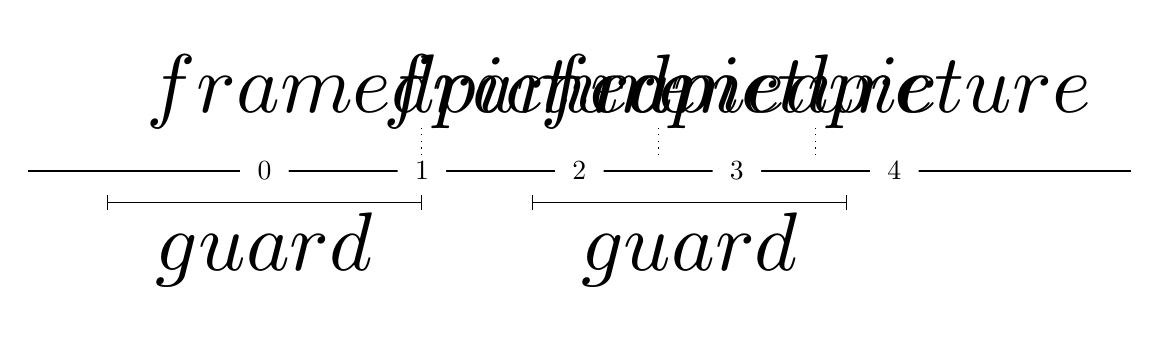
\begin{tikzpicture}
	\draw (-3,0) -- (11,0);
	\begin{scope}[every node/.style={circle, fill=white}]
		\node at (0,0) {$0$};
		\node at (2,0) {$1$};
		\node at (4,0) {$2$};
		\node at (6,0) {$3$};
		\node at (8,0) {$4$};
	\end{scope}
	\begin{scope}[every node/.style={scale=3}]
		\foreach \p in {2,5,7} {
			\node at (\p,1) {$\texttwemoji{framed picture}$};
			\draw[dotted] (\p,0.2) -- (\p,0.6);
		}
		\foreach \g in {0,5.4} {
			\node at (\g,-1) {$\texttwemoji{guard}$};
			\draw[|-|] (\g-2,-0.4) -- (\g+2,-0.4);
		}
	\end{scope}
\end{tikzpicture}
\end{center}

Note that there are many satisfactory ways to position these two guards while still protecting all three paintings, but you cannot protect all three with only one guard.

\begin{enumerate}
\item The art gallery also presents Larry with one potential strategy to protect the paintings:

\textit{Place a guard one unit to the left of the leftmost unprotected painting, and repeat.}

Provide a counterexample to show that the proposed strategy does not necessarily minimise the number of guards used.

\item Help Larry modify the art gallery's algorithm to make it correctly minimise the number of guards used; then, analyse the time complexity and prove the correctness of your algorithm.

\textbf{Hint:} \emph{One method to prove correctness of greedy algorithms is \emph{Greedy Stays Ahead}. Here, ``ahead" can be determined by the number of paintings protected by the first $k$ guards.}
\end{enumerate}
\end{question}

\clearpage

\begin{rubric}
\begin{enumerate}
    \item  Provide a clear and concise counterexample to the provided algorithm. This should include the number of paintings $n$ (which should be no more than four), the positions of the paintings $[p_1, \cdots, p_n]$, the number of guards the provided strategy would choose, and a satisfactory placement of fewer guards.
    \item Examples given in the lectures will be useful in the proof.

\end{enumerate}
\expected[2]{three sentences, a page.}
\end{rubric}
\clearpage
\begin{solution}
    % Write your solution here.
\end{solution}
\begin{attribution}
    % Write any attributions here.
\end{attribution}
\end{document}